%%% Copyright (C) 2018 Vincent Goulet
%%%
%%% Ce fichier fait partie du projet
%%% «Rédaction avec LaTeX»
%%% http://github.com/vigou3/formation-latex-ul
%%%
%%% Cette création est mise à disposition selon le contrat
%%% Attribution-Partage dans les mêmes conditions 4.0
%%% International de Creative Commons.
%%% http://creativecommons.org/licenses/by-sa/4.0/

\section{Organisation d'un document}

\begin{conseil}
  Utilisez impérativement les commandes {\LaTeX} pour identifier les
  différentes parties (la structure) d'un document.
\end{conseil}

\subsection{Parties d'un document}

\begin{frame}[fragile]
  \frametitle{Titre et page de titre}
  {\LaTeX} peut composer une page de titre automatiquement à partir
  des informations pertinentes.

  \begin{lstlisting}
%% préambule
\title{`\meta{Titre du document}'}
\author{`\meta{Prénom Nom}'}
\date{`\meta{31 octobre 2014}'} % automatique si omis

%% corps du document
\maketitle
  \end{lstlisting}
\end{frame}

\begin{frame}[fragile=singleslide]
  \frametitle{Sections}
  \begin{itemize}
  \item Découpage du document en sections
\begin{lstlisting}
\part{`\meta{titre}'}
\chapter{`\meta{titre}'}
\section{`\meta{titre}'}
\subsection{`\meta{titre}'}
\end{lstlisting}
\begin{lstlisting}
\subsubsection{`\meta{titre}'}     % à éviter dans un livre
\end{lstlisting}
\begin{lstlisting}
\paragraph{`\meta{titre}'}         % jamais (?) utilisé
\subparagraph{`\meta{titre}'}      % idem
\end{lstlisting}
  \item Numérotation automatique
    \begin{demo}
      \begin{minipage}{0.45\linewidth}
\begin{lstlisting}
\section{Hypothèses}
\end{lstlisting}
      \end{minipage}
      \hfill
      \begin{minipage}{0.45\linewidth}
        
\includegraphics[height=0.8\baselineskip,keepaspectratio]{section-num}
      \end{minipage}
    \end{demo}
  \item Sans la numérotation
    \begin{demo}
      \begin{minipage}{0.45\linewidth}
\begin{lstlisting}
\section*{Hypothèses}
\end{lstlisting}
      \end{minipage}
      \hfill
      \begin{minipage}{0.45\linewidth}
        
\includegraphics[height=0.8\baselineskip,keepaspectratio]{section-non-num}
      \end{minipage}
    \end{demo}
  \end{itemize}
\end{frame}

\begin{frame}[fragile=singleslide]
  \frametitle{Annexes}

  Les annexes sont des sections ou des chapitres avec une numérotation
  alphanumérique (A, A.1, ...)
  \begin{itemize}
  \item \cs{appendix} identifie les sections suivantes comme des annexes
  \item Dans le titre, «Chapitre» changé pour «Annexe» le cas échéant
  \end{itemize}
\end{frame}

\begin{frame}[fragile=singleslide]
  \frametitle{Table des matières}

  La commande \cs{tableofcontents} produit automatiquement la table
  des matières.

  \begin{itemize}
  \item Requiert plusieurs compilations
  \item Sections non numérotées pas incluses
  \item Avec \pkg{hyperref}, produit également la table des
    matières du fichier PDF
  \item Classe \class{memoir} fournit \cs{tableofcontents*} qui
    n'insère pas la table des matières dans la table des matières
  \end{itemize}
\end{frame}

\subsection{[~Exercice~]}

\begin{exercice}
  Utiliser le fichier \fichier{exercice\_parties.tex}.

  \begin{enumerate}
  \item Étudier la structure du document dans le code source.
  \item Ajouter un titre et un auteur au document.
  \item Créer la table des matières du document en le compilant 2 à 3
    fois.
  \item Insérer deux ou trois titres de sections de différents niveaux
    dans le document.
  \item Vous remarquerez que la numérotation cesse à partir des
    sous-sections. C'est une particularité de la classe
    \class{memoir}.

    Recompiler le document après avoir ajouté au préambule la commande
\begin{lstlisting}
\maxsecnumdepth{subsection}
\end{lstlisting}
  \item Ajouter une annexe au document.
  \end{enumerate}
\end{exercice}

\subsection{Renvois automatiques}

\begin{frame}
  \frametitle{Étiquettes et renvois automatiques}

  Ne \alert{jamais} renvoyer manuellement à un numéro de section,
  d'équation, de tableau, etc.

  \begin{itemize}
  \item «Nommer» un élément avec \cs{label}
  \item Faire référence par son nom avec \cs{ref}
  \item Requiert 2 à 3 compilations
  \end{itemize}
\end{frame}

\begin{frame}[fragile=singleslide]
  \frametitle{Exemple (code source)}

  \begin{lstlisting}[emph={\label,\ref}]
\section{Définitions}
\label{sec:definitions}

Lorem ipsum dolor sit amet, consectetur
adipiscing elit. Duis in auctor dui. Vestibulum
ut, placerat ac, adipiscing vitae, felis.

\section{Historique}

Tel que vu à la section \ref{sec:definitions},
on a...
\end{lstlisting}
\end{frame}

\begin{frame}
  \frametitle{Exemple (résultat)}

  \fbox{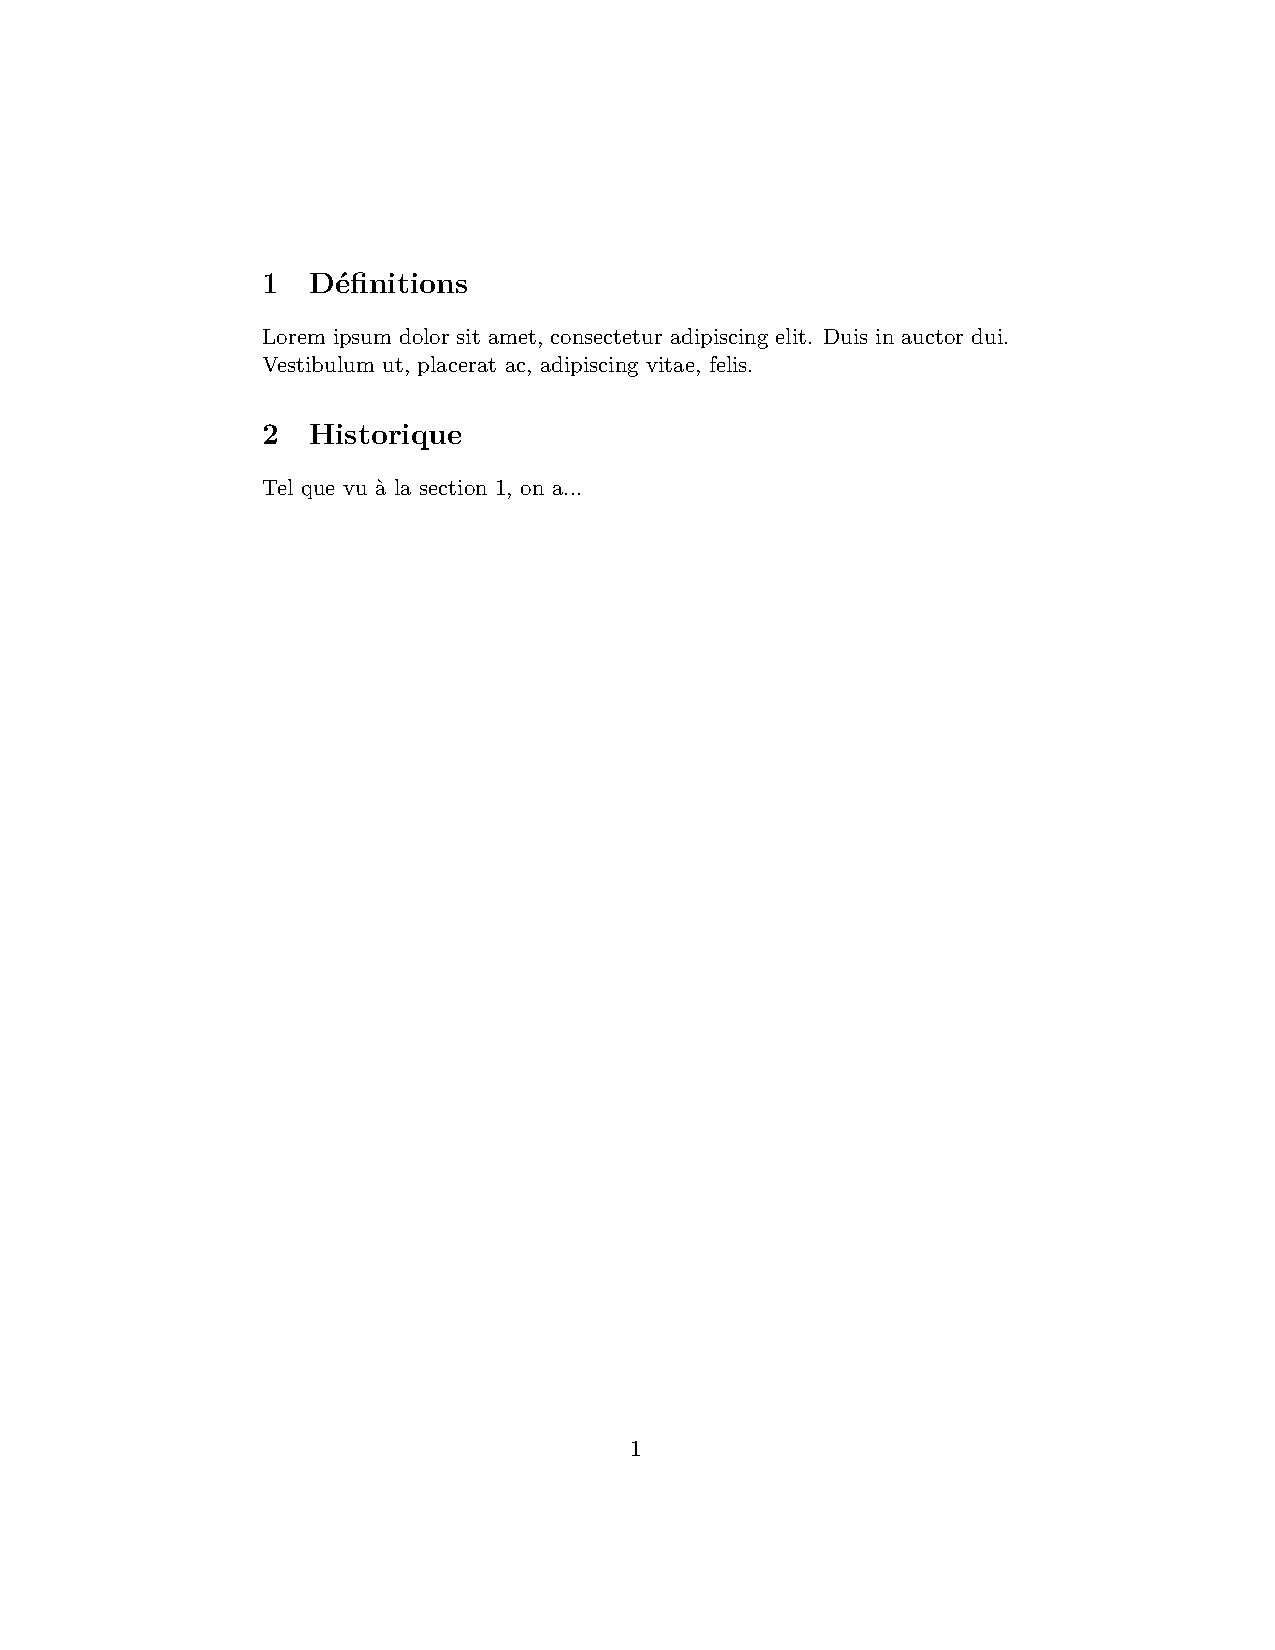
\includegraphics[viewport=124 550 484 664,clip=true,width=0.98\linewidth]{exemple-renvoi}}
\end{frame}

\subsection{[~Exercice~]}

\begin{exercice}
  Utiliser le fichier \fichier{exercice\_renvois.tex}.
  \begin{enumerate}
  \item Insérer dans le texte un renvoi au numéro d'une section.
  \item Activer le paquetage \pkg{hyperref} avec l'option
    \texttt{colorlinks} et comparer l'effet d'utiliser \cs{ref} ou
    \cs{autoref} pour le renvoi.
  \end{enumerate}
\end{exercice}

%%% Local Variables:
%%% TeX-master: "formation-latex-ul-diapos"
%%% TeX-engine: xetex
%%% coding: utf-8
%%% End:
